\documentclass[10pt, conference, compsocconf]{IEEEtran}

\usepackage{cite}
\usepackage{graphicx}
\usepackage[cmex10]{amsmath}
\interdisplaylinepenalty=2500
\usepackage{array}
\usepackage{mdwmath}
\usepackage{mdwtab}
\usepackage[caption=false,font=footnotesize]{subfig}
\usepackage{fixltx2e}
\usepackage[utf8]{inputenc}

\hyphenation{op-tical net-works semi-conduc-tor na-tur-al}

\begin{document}

\title{Using High-Level Languages in Hard Real-time Embedded Systems:\\a Case Study with the Lua Programming Language}

\author{\IEEEauthorblockN{Alex de Magalh\~{a}es Machado, Ant\^{o}nio Augusto Fr\"{o}hlich}
\IEEEauthorblockA{Laboratory for Software and Hardware Integration (LISHA)\\
Federal University of Santa Catarina (UFSC)\\
88040-900 Florian\'{o}polis - SC - Brazil\\
\{alex,guto\}@lisha.ufsc.br}
}

\maketitle

\begin{abstract}
Virtual machine-based high-level languages have been increasingly used in embedded systems. Their virtual machine provides several abstractions that ease applications development. To achieve that, large run-time support systems must be provided. However, embedded systems can hardly afford necessary resources. Also, most of these virtual machines are not suitable for real-time computing. Our goal is to reduce this gap between these high-level languages and hard real-time embedded systems. In previous work, we ported the virtual machine of the Lua programming language to the Embedded Parallel Operating System. In this paper we describe our work to support real-time applications in Lua. We attained to enable real-time computing through a small, powerful, and user-friendly programming language. We present a case study that successfully achieved real-time behavior and satisfied the constraints. Nevertheless, we discuss the challenges we found and the improvements we are looking forward to implement.

\end{abstract}

\begin{IEEEkeywords}
Embedded system; Real-time; Virtual machine; High-level language; Lua;

\end{IEEEkeywords}

\section{Introduction}
The employment of virtual machine-based high-level languages can considerably improve applications development. They usually use natural language constructions that are easily recognizable by developers and also hide details from the underlying hardware, such as memory access model, management of scope and processor instruction set. This is done by creating abstractions that are easy for developers to understand and are also powerful enough to do these computations without user intervention. These abstractions make high-level languages user-friendly and are also responsible for the improved application development, which leads to cost and time-to-market reduction.

As examples of these abstractions, we could mention garbage collection, multi-threading, complex and powerful data structures, object-oriented programming, powerful Application Programming Interfaces, and so on. In order to make these abstractions work properly, large run-time support systems must be provided. This run-time environment usually consists of an operating system, with support for device drivers, libraries, and virtual machines. One advantage of virtual machines is that they also improve portability, flexibility, and security. For these reasons, virtual machine-based high-level languages require much more resources than low-level languages or even other high-level languages.

On the other hand, embedded systems are the ones that provide fewer resources for their applications. Virtual machine-based high-level languages seldom meet the requirements of real embedded systems. However, embedded systems could take advantage of the usage of such high-level languages. Using these languages makes it easier to write better programs, with fewer errors, in less time and with less efforts~\cite{Carro:2006}. For instance, embedded systems do not usually interact with humans, and they need to be robust enough to stay operating even in the event of an error. Also, their time to market must be minimized so they can be competitive.

The interoperability between virtual machine-based high-level languages and embedded systems has even more issues when it comes to hard real-time embedded systems. These systems are characterized by predictable behavior. The language implementation and its underlying support must provide enough information so designers can predict their application's execution time, in order to guarantee that it will always meet its time constraints. However, because of the abstractions the run-time support system provides, designers may not know how some of the functionalities are being executed, and therefore cannot make predictions on execution behavior. This is an issue for every hard real-time system, but virtual machine-based high-level languages normally make it more critical.

This disparity makes it difficult to accomplish the use of these high-level languages in hard real-time embedded systems. Our goal is to reduce this gap between them. There are already several approaches that tackle this problem, and they accomplished much in different fields. One of the biggest steps towards this objective is the constant improvement in hardware resources. Micro-controllers are increasingly providing more resources, which is essential to the improvement of their software counterparts. Newer compile-time optimizations are also enabling high-level languages to run fast enough to be compared to low-level languages. However, henceforth, when we speak of high-level languages, we mean virtual machine-based high-level languages, which are the focus of our work and cannot afford many of these optimizations.

We chose the Lua programming language as our high-level language because of its advantageous lightweight virtual machine. Lua applications are executed using the Lua Virtual Machine (LVM). This virtual machine has features that make it easy to attain a soft real-time support, which makes it suitable for games development. However, it does not support hard real-time applications, and this makes it unsuitable for a large amount of embedded systems. We already ported the LVM to the Embedded Parallel Operating System (EPOS) in a previous work~\cite{Epos:2010}~\cite{Machado:2010}. Instead of creating an LVM from the beginning, we changed the existing LVM in order to make it suitable for embedded systems, so our LVM works the same way as its desktop counterpart.

In this paper we report the improvement we have done in our virtual machine in order to support hard real-time applications. Predictability is the main concern in terms of real-time computing and the LVM has features that are hard to predict. For instance, the LVM uses a Garbage Collector, and it is difficult to know how much memory it is going to deallocate in every cycle, and how much time it will take to do it. Also, Lua has tables that dynamically grow depending on how they are being used, and it is hard to know when they are going to request more memory. Therefore, we present all the challenges we found, how we solved them, and what could be done to improve our LVM. A case study is described in order to show our implementation in a real application.

The rest of the paper is organized as follows. Section 2 describes related works on real-time embedded virtual machines and on interoperability between high-level languages and embedded systems. Section 3 describes our embedded LVM. All the adaptations we had to do in order to support it on an embedded system are briefly discussed. Section 4 presents all the challenges in supporting hard real-time applications in Lua and how we managed to solved them. In Section 5 we describe our case study with a real application and we evaluate its real-time behavior. Section 6 addresses limitations of our approach, describes how our work could be improved, and reports future works.

\section{Related Work}
Tools for compile-time analysis, verification, specialization, and low-level optimization can be used to reduce the gap between high-level languages and embedded systems~\cite{Carro:2006}, but we decided to work with virtual machines because of other advantages such as portability, flexibility, and security. With more resources being provided by hardware, more powerful operating systems are created, and more complex applications are developed. This operating systems may include databases, agents, and application driven or message-oriented systems, but also virtual machines~\cite{Costa:2007}.

In the realm of virtual machines, there are different approaches: virtualizing real hardware, virtualizing intermediate program representation and virtualizing bytecode interpretation~\cite{Costa:2007}. We are focusing our efforts in virtual machines for bytecode interpretation. Some of these virtual machines replace the entire operating system and others complement the operating system~\cite{Costa:2007}, but they have common characteristics. Both of them support one (usually Java) or a few high-level languages and were designed to suit specific types of applications or to run on specific platforms. The embedded LVM is a language-specific virtual machine that adds new functionalities to EPOS. 

There are several approaches for virtual machines in embedded systems and their different behaviors are better described in our previous work~\cite{Machado:2010}. There are also various approaches to hard real-time virtual machines. They all have to care about the problem of predictable execution, and scheduling and garbage collection are reasons why this prediction is difficult to achieve~\cite{Marcondes:2009},~\cite{Chang:2006}.

Most of the approaches focus on the Java programming language and its Real-time Java Specification (RTJS). This RTJS allowed the implementation of several real-time Java virtual machines, although it leaves many important problems unaddressed~\cite{Auerbach:2007}. The implementation of the RTJS on the Ovm Java virtual machine offered better portability and productivity over a traditional language such as C++ and complex issues were properly solved~\cite{Armbruster:2007}. The J9 Java virtual machine applies an appropriate garbage collector and provides a complete implementation of the RTJS~\cite{Auerbach:2007}. Anyhow, these implementations are not suitable for small embedded devices, with less than 100KB available for non-volatile memory. In fact, the majority of works on real-time Java virtual machines do not even address the possibility of usage in such devices.

\section{Lua on EPOS}

The LVM is a middleware level virtual machine for bytecode interpretation. In this scenario, high performance may be attained by implementing an execution model that closely resembles an actual hardware. The LVM does that through register-based bytecode interpretation. Also, there are usually similarities between what virtual machines provide for their applications and what the operating system provides for the virtual machines. The implementation of a virtual machine could be optimized to allow applications to directly use the feature from the operating system, which enhances performance. That was our goal when we ported the LVM to EPOS.
 
Lua is one the fastest in the realm of interpreted scripting languages~\cite{Ierusalimschy:2007}. It has a powerful syntax along with consistent and intuitive semantics. Its C API is small and flexible, and the whole run-time support fits into 128 KB of ROM and 64KB of RAM. Lua applications are compiled at run-time by its virtual machine. To execute Lua applications on EPOS, a simple stand-alone interpreter was created and defined as an EPOS application. Through the C API, this application opens the virtual machine and sends the Lua application source code to the LVM. A Lua State is created and the LVM compiles the Lua application. Finally, the EPOS tells the LVM to execute the application, and keeps waiting for its finalization.

Embedded operating systems usually feature adequate run-time support for most applications, turning the problem of adapting the LVM to EPOS into interface adaptation along with proper language configuration. Existing embedded virtual machines are usually a subset of a general-purpose virtual machine for desktop systems. These subsets do not mostly provide features that are hard to implement on small embedded systems. Although we also create a subset of the LVM, only unnecessary features were removed, such as functions for accessing environment variables and external commands. Moreover, the main use for software localization tools in the LVM is to provide software localization for Lua applications, but such tools are not used in embedded systems, and therefore were removed. Currently, EPOS can only run one Lua script at a time, so the Lua Package Library was also disabled.

To give a shape to the remaining features, we defined a Lua profile, in which we create a set of lower level programming interfaces with available resources for the embedded version of the LVM. This Lua profile aims to help Lua developers to understand the functionalities LVM provides for embedded Lua applications.

This section briefly describes our approach to port the LVM to EPOS, which is a multi-platform real-time operating system for embedded systems, designed to guide and provide architecture transparency to the development of scenario independent component families~\cite{Marcondes:2009}. These component families can then be used in different environments through applying aspect programs~\cite{Frohlich:2001},~\cite{Cancian:2007}. EPOS is designed for embedded hardware and provides most of the support Lua needs to work. However, Lua uses C standard libraries that are not present in EPOS. We could add these libraries to the environment and most of it would work properly, but we would be also adding unnecessary code. We therefore chose to implement only the functions Lua needs.

We defined our Lua Profile to standardize the minimum support an embedded device must provide to proper LVM execution. This profile specifies hardware requirements, required changes in the virtual machine and in the language itself and which libraries are available for applications. Ideally, a profile is only a subset, so embedded Lua applications should also work on desktop implementations of the virtual machine. Our hardware requirements consist of only memory requirements. Any type of hardware platform may be used to support Lua applications. In terms of memory, designers have to provide a minimum of 144KB of non-volatile memory and 32KB of volatile memory for proper execution of the LVM. These requirements take into account the memory utilization by the operating system, the LVM itself, and its libraries.

The Lua programming language was not changed in our profile, but some modifications were made to the virtual machine. Table \ref{profile} depicts the libraries and functions supported in our Lua profile. In order to properly create an efficient and maintainable Lua runtime environment for embedded systems, we need to make clear what LVM provides and what Lua applications need. Even if a feature is supported by EPOS and LVM, it is possible that it will never be used by a Lua application running on EPOS. This issue is solved by the employment of our Lua Profile, which defines a subset of functionalities that LVM provides for embedded Lua applications.

\begin{table*}[!t]
\caption{Libraries supported by our Lua profile}
\label{profile}
\centering
\begin{tabular}{|c|c|c|c|c|}
\hline
Basic Library & Table Library & OS Library & String Library & Mathematical Library \\
\hline
assert , error & concat & clock & byte & abs \\
collectgarbage & insert & date & char & acos , asin \\
getfenv & maxn & difftime & dump & atan , atan2 \\
getmetatable & remove & exit & find & cell , floor \\
ipairs , pairs & sort & time & format & cos , sin \\ 
load , loadstring & & & gmatch & cosh , sinh \\ \cline{2-3}
next & I/O Library & Coroutine Library & gsub & deg \\ \cline{2-3}
pcall , xpcall & close & create & len & exp \\
print & flush & resume & lower , upper & fmod \\
rawequal & read & running & match & frexp , ldexp \\
rawget , rawset & type & status & rep & log , log10 \\
select & write & wrap & reverse & max , min \\
setfenv & & yield & sub & modf \\
setmetatable & & & & pow \\
tonumber & & & & rad \\
tostring & & & & random \\
type & & & & randomseed \\
unpack & & & & sqrt \\
 & & & & tan , tanh \\
\hline
\end{tabular}
\end{table*}

\section{Hard Real-time Support}
Lua is used for several different kinds of applications, but the most common use is in games development. In this field, applications usually have time constraints, as they need to process more than 30 frames per second. However, it is acceptable that the application sporadically miss these time constraints. In such cases, one or a few frames are omitted, and the application continues to execute soundly. Lua does not guarantee that only a few frames will be omitted, but its implementation attained to reduce the probability that this will happen. However, designers have a much more complex situation when it comes to hard real-time applications. Therefore, henceforth, when we mention real-time applications, we mean hard real-time applications, which are the focus of this discussion.

We call them hard real-time applications because they shall never miss their deadlines, since their real-time tasks are mission critical. Missing this deadline is unacceptable and useless. Several analyses have to be performed in order to assure the determinism of the real-time tasks. In other words, designers must predict the application's worst-case execution time (WCET). After that, they can be sure the application will never spend more time than its WCET performing its tasks. In this scenario, both operating system and virtual machine must provide predictable behavior as well.

It is more difficult to predict the behavior of the real-time tasks when it comes to high-level languages. The way these abstractions are being executed is not always clear and this eventually turns real-time applications impractical in some high-level languages. In terms of the Lua programming language, real-time applications are also impractical by default. However, it is possible to adjust the virtual machine in order to enable them. In this section we clarify the problems in supporting real-time applications in Lua, what are the possible solutions, and which solution we chose for our case study.

\subsection{Scheduling and Memory Allocation}
Tasks scheduling is a major subject in real-time applications~\cite{Marcondes:2009}. A scheduler for real-time operating systems must guarantee that all the real-time tasks meet their deadlines. This issue can be solved by proper scheduling policies, such as a priority-based scheduler~\cite{Armbruster:2007},~\cite{Auerbach:2007}. Nevertheless, Lua does not support multi-threading, i.e. its threads cannot be dynamically scheduled.

EPOS, however, supports multi-threading. EPOS threads may be executing along with the LVM and real-time schedulers were already created for it~\cite{Marcondes:2009}, but the LVM runs on EPOS in a single thread. For our case study, we expect that it is the only thread running on the system in order to guarantee its real-time behavior. This way, the LVM interpreter is always executing in the processor.

However, an off-line scheduling is still needed. For instance, if a Lua Thread A creates a new Thread B and requires its execution, Thread A will have to wait Thread B to finish or voluntarily stop its execution. If Thread A executes a real-time task, the application designers must guarantee that Thread B will finish in time, in order to allow Thread A to continue its execution.

Most traditional memory allocators are unpredictable. Some dynamic memory allocators for real-time systems have been proposed~\cite{Masmano:2004}. The LVM allows us to define our own custom allocator, and therefore we used EPOS allocator, which is appropriate for real-time applications.

\subsection{Dynamic Tables}
An exclusive issue with the Lua programming language is Tables, its main data structure. Tables in Lua have an array part and a hash part. For example, if developers want to create an array, the hash part stays empty and data is stored in the array part. A Table may have data stored in both parts at the same time. However, the problem with Tables is that they dynamically grow. Developers can create an empty Table and then insert values in it one at a time, or they can create it with a few elements and then add a new element, forcing the Table to grow. It is invisible for developers, but it is subject that has to be taken into account in real-time applications.

Possible solutions would be disabling Tables or impeding them to grow. Disabling Tables is infeasible because they are Lua's only complex data structure, and impeding them to grow would negatively impact applications development, since it is a facility that would not be available any more. Also, determining fixed sizes to Tables would require several changes in the entire virtual machine, since its syntax. Although it is invisible for Lua developers, however, this growth can be predicted. Developers must know that when they are affecting a table's length, they are possibly making it to grow.

A Table in Lua usually grows when its users try to insert a value in a position not known to exist before. Such operation would cause an error in many other programming languages, but it is natural in Lua. In terms of our case study, the prediction of the WCET took into account that any time when a value is being inserted on a table, the table is probably growing in order to store that value.

\subsection{Garbage Collection}

In high-level languages, a Garbage Collector is normally provided. A Garbage Collector allows developers to not care about memory deallocation when they are programming, and hence it is known for improving applications development. It is one of the complex abstractions Lua also provides, and it is the biggest problem with real-time applications in Lua. Garbage Collectors are normally unpredictable because the maximum time they spend deallocating memory is unknown.

The Lua Garbage Collector has improved through the years to a incremental mark-and-sweep Garbage Collector, which has been described in details in some works~\cite{Ierusalimschy:2007},~\cite{Barros:2008}. With the right management by developers, it can be appropriate for soft real-time applications, because of its incremental algorithm. This Garbage Collector has an API that allows developers to control some simple aspects of its execution during run-time (e.g. stop, restart, perform a complete cycle, perform only some work, get current memory usage). Disabling the Garbage Collector solves the problem, but it is impractical depending on the application.

Besides those functions, it also provides two functions to control the time between two Garbage Collector execution cycles and the time a Garbage Collector cycle lasts, called 'setpause' and 'setstepmul'. The former accepts a pause percentage p as its parameter, and given that Lua is using m bytes of memory, it waits until Lua is using m*p bytes to start a new cycle. This way, a pause of 100\% makes a new cycle to start as soon as possible, and a pause of 200\%, which is the default, waits for memory usage to double before starting a new cycle. For the latter function, which also receives a percentage as its parameter, values smaller than 100\% make the collector so slow it could never finish a cycle, and huge values make it work such as a non-incremental Garbage Collector~\cite{Ierusalimschy:2006}.

To predict the cost of a Garbage Collector, two times must be known: the rate at which a Garbage Collection cycle happens and the WCET of a Garbage Collection cycle. With those two Lua API functions, these two times may be calculated. For the former, with minor changes to the EPOS allocation function, it is possible to keep count on allocated memory, and then it is possible to predict the frequency of Garbage Collection cycles. For the latter, the time spent deallocating memory of each different Lua object must be known.

Knowing how much memory and how much time it takes to deallocate that memory is the key to know how much time the Garbage Collector takes to execute at the worst-case situation. This way, Lua developers can determine their application execution time even taking into account the Garbage Collection. Successful works have been done in order to predict the Garbage Collection's WCET in Java Virtual Machines~\cite{Auerbach:2007},~\cite{Chang:2006}, and the cost of a incremental mark-and-sweep Garbage Collector specifically has already been modeled in related works and it is feasible for Lua as well~\cite{Fu:2007}.

In our case study, we do not use the 'setpause' function. We do not determine the pause between two Garbage Collector cycles in terms of memory usage. Instead, a Garbage Collector cycle is performed after every iteration of the Lua application, so an entire application cycle is our pause between two collection cycles. In other words, the Garbage Collector stays disabled during the execution of the real-time tasks, guaranteeing real-time behavior. The values for the 'setstepmul' function depend on how much time the Garbage Collector is allowed to execute and how much memory needs to be deallocated, so it may vary from one application to another. In our case study, we used default values.

\section{Evaluation}
Our hard real-time support was evaluated through a case study with a simple Lua application. We determined a WCET of 100ms for our evaluation. The application is an implementation of the Quicksort algorithm, which is part of a test application deployed with the source code of the original implementation of Lua. We chose a sorting algorithm because it allows us to stress tables usage and Garbage Collection execution. The application receives 1000 or less elements and inserts them into an array, and then it sorts the array. During these steps, the Garbage Collector stays disabled. When the array is sorted, if there is still time left for some more work, the Garbage Collector is resumed and it executes at least one collection step and at most one collection cycle, depending on how much time is left and on how the 'setstepmul' function is being used.

Since the LVM is the only thread executing on EPOS and the Garbage Collector stays disabled, the execution time of our application depends on the array size and on how much time it takes to allocate memory. The worst-case scenario is when the array has 1000 elements, since this is the maximum amount of elements it can have. With 1000 elements, the table used to store the array will grow 1000 times, and an array with 1000 elements will be sorted.

We guarantee that the memory allocator is appropriate for real-time applications, and therefore an upper bound of the application's execution time can be determined, which assures the predictability we need to run real-time applications. This upper bound considers an array with length 1000, since it is the worst-case scenario, and sorting this array must take at most 100ms.

All of our execution times were obtained at I/O ports with an oscilloscope. In order to simplify our evaluation, we consider as real-time tasks only the actual application execution. This is the most critical part, since embedded systems applications usually run for a long time period. Also, these applications do not normally restart, so loading libraries, opening and closing the virtual machine and compiling the Lua application are tasks normally done only once. Hence our tests only show the time spent executing the actual Lua application.

Figure \ref{performance} shows its execution time. We tested two different configurations. In the first one, the sorted arrays had random amount of elements. After several iterations, the average size of the sorted arrays was 485 elements. In this scenario, the application executed in 45.78ms, which is 45.78\% of the WCET, as showed in Figure \ref{performance}. The standard deviation was 18.51ms and the coefficient of variation was 0.4. Our tests showed that our application took less time to execute than it could. This way, the Garbage Collector was able to perform a whole collection cycle in all of our tests.

In fact, the execution times depicted in Figure \ref{performance} already took into account the time spent by the Garbage Collector. However, an entire collection cycle took only 0.98ms, which is not much significant. Still, the Garbage Collector was able to always maintain memory usage below 42KB for this specific application. Without any Garbage Collection the memory usage would be almost 600KB after 100 iterations.

In the second scenario, the algorithm always had to sort an array with 1000 elements, which is the worst-case situation. In this scenario, the application's execution time was higher, as we already expected, but it was still lower than the upper bound. The application spent only 91.83ms executing, which is also 91.83\% of the WCET. The standard deviation was 5.7ms and the coefficient of variation was 0.06. The time spent exclusively by the Garbage Collection was only 1.03ms.

\begin{figure}[!t]
\centering
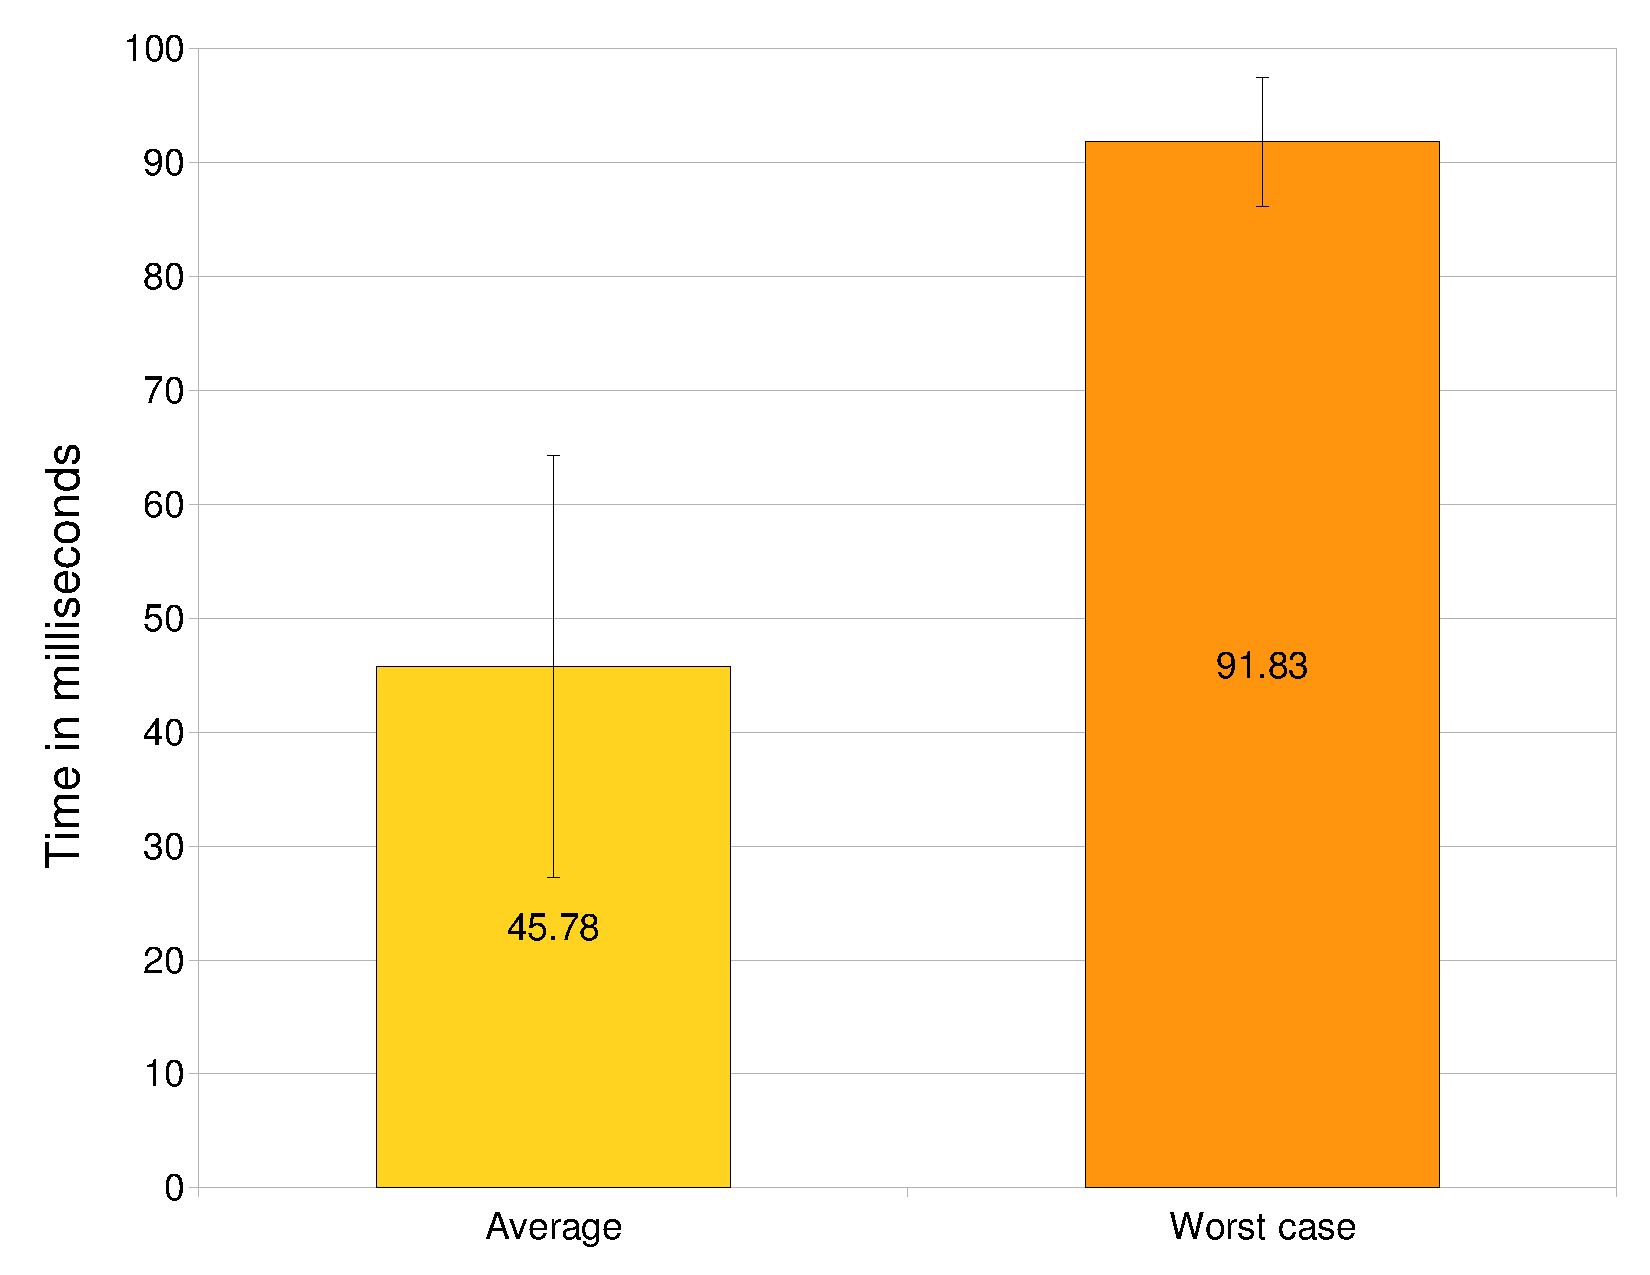
\includegraphics[width=\columnwidth]{fig/performance}
\caption{Execution times of the application taking into account arrays with random size and also arrays with worst-case size}
\label{performance}
\end{figure}

At last, we also measured the EPOS size with the LVM, the necessary libraries and the Lua application. Figure \ref{size} shows these values. Although the final system has more than 132KB, it is a small size considering that we support a virtual machine-based high-level language with hard real-time support. With less than 100KB it is possible to support Lua applications without using libraries, so a simple real-time application could use less then 100KB. We also noticed that the LVM needed less than 42KB of volatile memory in order to perform these tasks, although we recognize it could require more depending on the application.

\begin{figure}[!t]
\centering
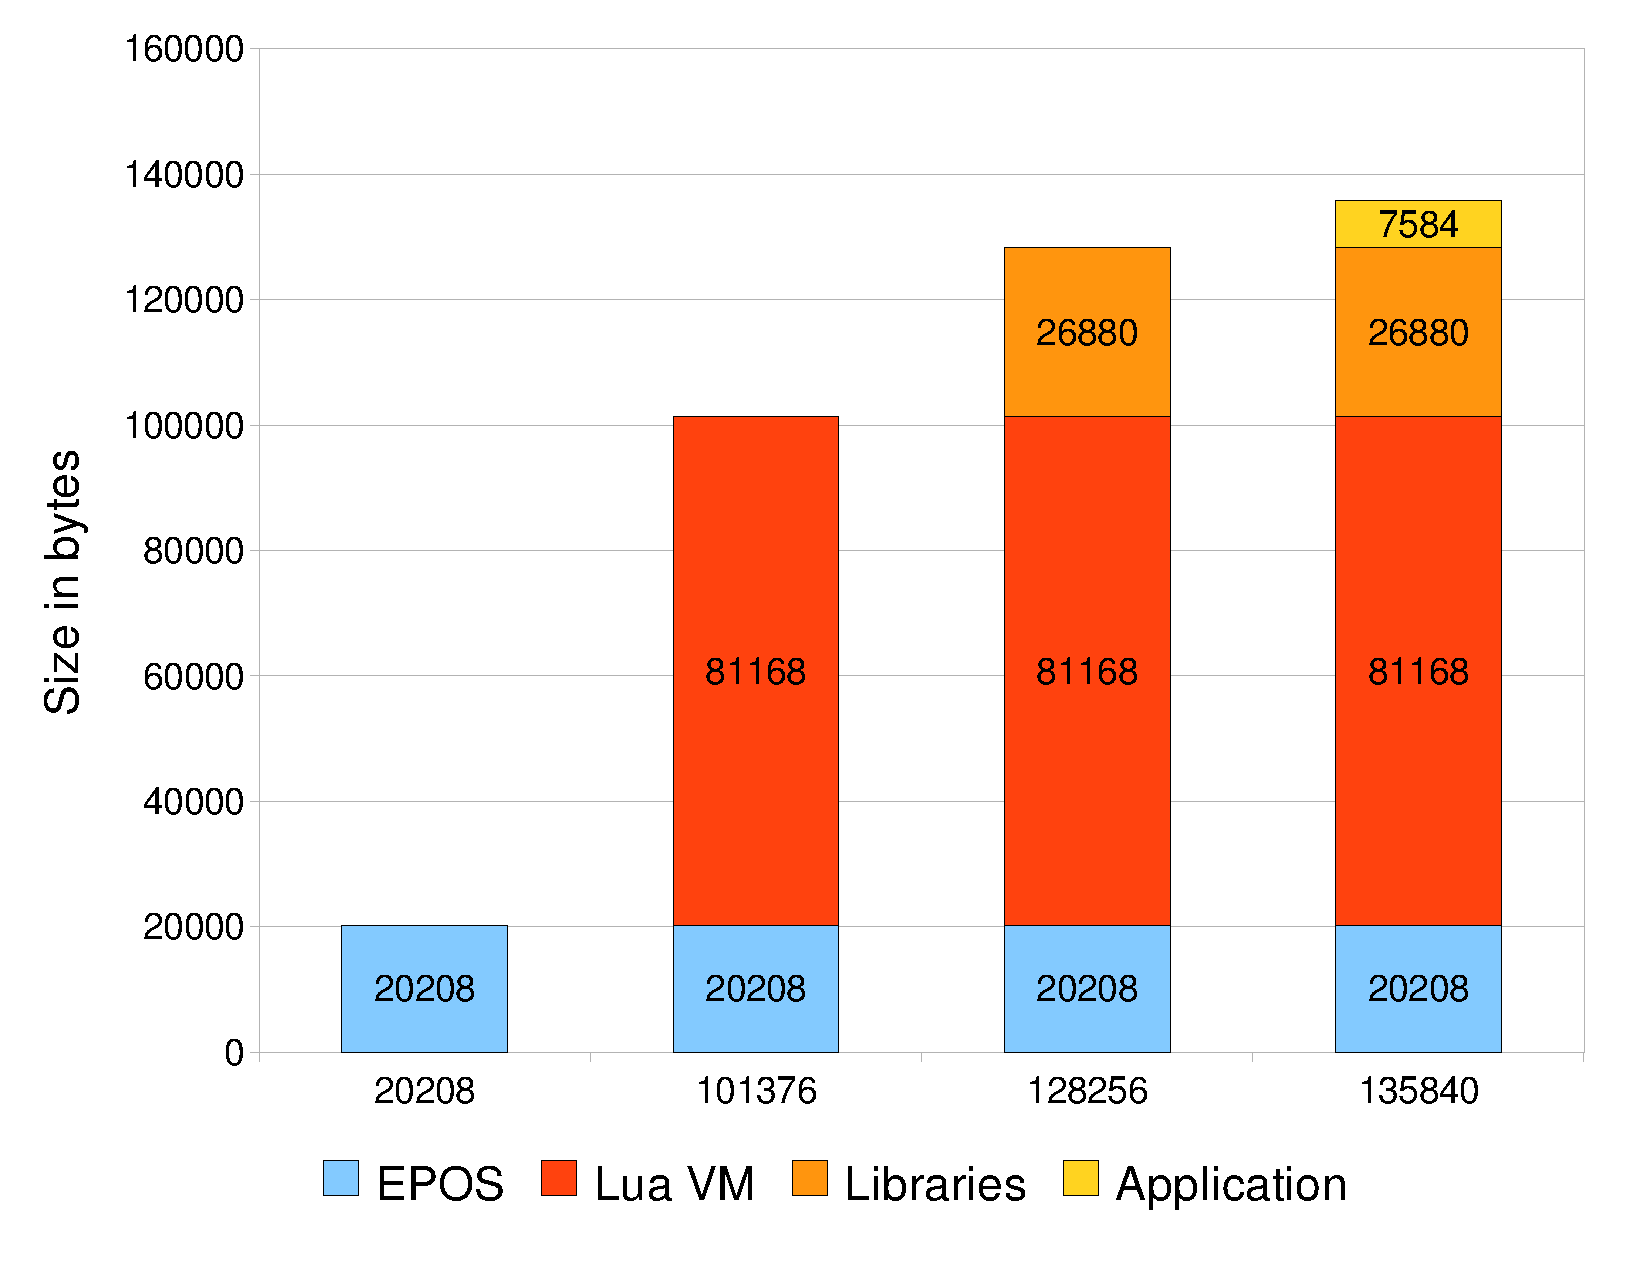
\includegraphics[width=\columnwidth]{fig/size}
\caption{EPOS size in different configurations}
\label{size}
\end{figure}

\section{Conclusion}
The use of the Lua programming language brings development improvement, portability and flexibility to the world of embedded systems, which reduces their time to market. A Lua Virtual Machine for EPOS achieved to reduce the gap between high-level languages and embedded systems. Our tests showed that Lua is a proper programming language for small embedded systems. It has a small footprint and satisfactory performance. Its virtual machine is small, portable and flexible. Its C API provides vast control over its virtual machine, even in terms of Garbage Collection.

In this paper we presented an improvement to the embedded Lua Virtual Machine, making possible the development of hard real-time applications in Lua. The point with real-time support is to assure predictability. We listed various problems with some virtual machine's features and we described our own solutions, although more could be done and we hope to encourage research in this subject with the solutions we discussed.

For instance, we simplified our analysis to a single thread model, where the LVM is the only thread executing on EPOS and using the default Lua coroutines. We are looking forward to map Lua threads into EPOS threads, enabling real multi-threading programming in Lua. If every aspect of the Lua programming language that affects real-time applications (e.g. Garbage Collection) were mapped into EPOS threads, a multi-threading-based schedulability model could be attained as a means to maintain the real-time support.

Also, the slightly unpredictable implementation of the Lua's Garbage Collector made us disable it during the execution of real-time tasks. After each iteration of the real-time tasks, we resume the Garbage Collector and allow it to perform one or a few collection steps, maintaining memory usage at a low level and assuring that the deadlines will still be met. Moreover, we solved the problem of dynamic tables using a proper memory allocator for real-time applications and always considering the WCET for all tables operations.

Hence we were able to create our first hard real-time Lua application, untangling tables behavior, controlling Garbage Collection and using a real-time operating system with real-time memory allocation and a single thread model of execution. The tests we executed showed that the LVM performed as we predicted.

Previous works reported that Lua is a fast scripting language, but we need to improve its performance in order to allow real deployment. Our future works will also focus on improvements for the Garbage Collector, so it executes inside the real-time tasks. This will enable shorter deadlines, which would make Lua to be suitable for a larger amount of real-time applications.

Efforts could be made to optimize some structural parts of the virtual machine core as well. The execution stack width, for example, was reduced in related works~\cite{Koshy:2009}. Although their virtual machine is different, similar optimizations could be tried. Some important structures could be optimized, such as 'GCObject' and 'TValue'. Efforts should be made to also assess such changes, because they can easily damage the LVM execution model. 

As we mentioned before, there are usually similarities between what virtual machines provide for their applications and what the operating system provides for the virtual machines. We achieved to optimize the virtual machine in order to allow applications to directly use some features from the operating system, but more features can be optimized this way. In terms of size, our embedded LVM does not really fit small embedded devices, although it is smaller than related works. We already somewhat optimized its size, but much more can be done. Actually, the very first step would be to take out of the EPOS system the application's compilation step. In the time of EPOS deployment, the Lua application can already be compiled and ready for execution. That would also improve performance of the system on EPOS, but it would mainly reduce the final system size.

We also looked for ways to bring our embedded LVM closer to real-time needs. The default Lua implementation has no support for real multi-threading and concurrency (i.e. Lua threads are cooperative). These abstractions could be implemented using EPOS native abstractions. EPOS supports multi-threading and has abstractions that support concurrency such as semaphore and mutual exclusion. New libraries can also be created for Lua. Some EPOS utilities already add new functionalities to EPOS native applications, and a Lua support for these utilities can enable their use in Lua applications.

\bibliographystyle{IEEEtran}
\bibliography{IEEEfull,highlevel,epos,vm,lua,realtime,gc}

%\IEEEtriggeratref{8}
% The "triggered" command can be changed if desired:
%\IEEEtriggercmd{\enlargethispage{-5in}}

\end{document}
